\documentclass[eng]{class}

% Publication Title
\title{Speech recognition}
% Short title for the header (copy the main title if it is not too long)
\shorttitle{Speech recognition}
       
% Authors
\author[1]{D. Ligari 518592}
% Author Affiliations
\affil[1]{Machine Learning course, University of Pavia, Department of Computer Engineering (Data Science), Pavia, Italy}
% Surname of the first author of the manuscript
\firstauthor{Ligari}
%Contact Author Information
\contactauthor{D. Ligari} % Name and surname of the contact author
\email{davide.ligari01@universitadipavia.it} % Contact Author Email
% Publication data (will be defined in the edition)
\publicationdate{\today}
% Place your particular definitions here
\newcommand{\vect}[1]{\mathbf{#1}}  % vectors
\github{https://github.com/DavideLigari01/speech-recognition.git}

\abstract{This report presents a lab activity focused on speech recognition. 
    The task is to recognize the pronunciation of a single word from a list of 35 words, using a multilayer perceptron. 
    The dataset used for the task is the Speech Commands Data Set, which includes 105,829 recordings of the 35 words, divided into training, validation, and test sets. 
    Feature extraction has already been performed, and the features are spectrograms that have been made uniform in size. 
    The lab activity encompasses various components, including the visualization of spectrograms, the application of feature normalization techniques, 
    training a multilayer perceptron without hidden layers, and exploring different network architectures.
     To gain insights into the network's performance, a confusion matrix is constructed to summarize its behavior, and classification errors are thoroughly analyzed. 
     The experiments are replicated using different feature normalization techniques, batch sizes and lambda values, in order to understand how these parameters affect the model's performance.}
\keywords{ MLP Neural network • Training • Speech recognition • Feature normalization • Confusion matrix • Spectrogram}
\date{\today}
% Start document
\begin{document}
\maketitle
\thispagestyle{FirstPage}

\pagenumbering{arabic}
\section{MLP Neural network}
\firstword{T}{he}
Multilayer Perceptron (MLP) neural network is a popular type of artificial neural network used in machine learning.
It consists of interconnected layers of nodes or neurons that process data to produce predictions.
MLPs employ activation functions, such as sigmoid, tanh, or ReLU, to introduce non-linearity and capture complex patterns.
By adjusting the weights of these connections through a process called backpropagation, MLPs can learn from data and make accurate predictions.
They are widely used in tasks like image recognition, speech processing, and natural language understanding.

\section{Visualize the data}
Gaining a deep understanding of the data being processed can greatly assist in designing an effective model.
With this goal in mind, Figure \ref{fig-1} presents the spectrogram of the initial training sample, providing a visual representation of the data.

\begin{figure}[h]
  \centering
  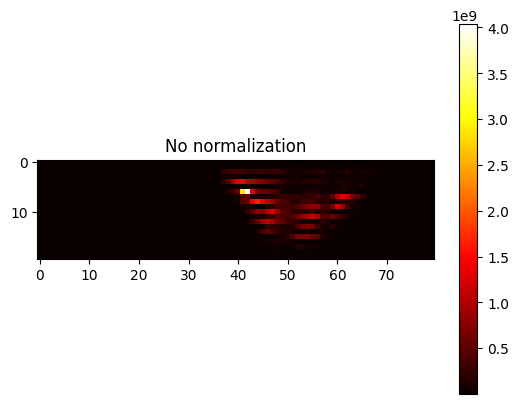
\includegraphics[width=.6\columnwidth]{images/sample_spectrogram.png}
  \caption{Spectrogram of a sample of the dataset}
  \label{fig-1}
\end{figure}
\section{Batch size selection}
Selecting an appropriate batch size is a critical factor in neural network training.
Opting for a higher value facilitates smoother convergence towards the minimum point;
however, each iteration becomes time-consuming as it needs to process a larger number of samples.
Conversely, a very low batch size can lead to unstable convergence, requiring more iterations.
On the positive side, each iteration is quicker since it processes only a limited number of samples.\newline
The figure below illustrates the test accuracy for different epochs and batch sizes in a model without hidden layers.
The model trained with a batch size of 10 exhibits gradual improvement but experiences oscillations.
Differently, the 200-sized batch demonstrates more consistent progress, albeit at a slower pace compared to the 50 and 100-sized batches.
Among these options, the 50-sized batch yields the highest accuracy, surpassing that of the 100-sized batch.
\begin{figure}[h]
  \centering
  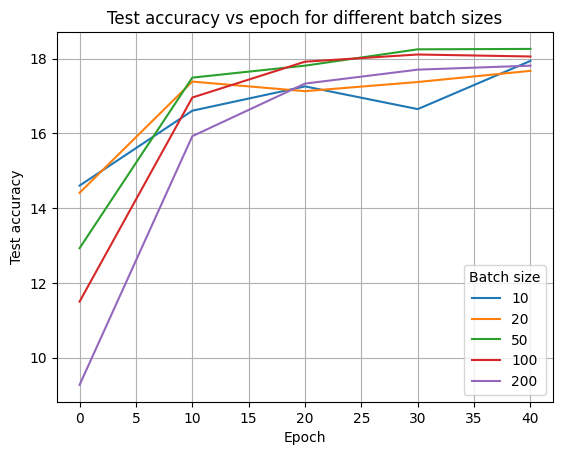
\includegraphics[width=.6\columnwidth]{images/batch_size.png}
  \caption{Test accuracy for different batch sizes}
  \label{fig-2}
\end{figure}

\pagestyle{OtherPage}
\section{Network architecture}
Numerous neural networks with varying depths and widths were trained to determine the optimal structure
and understand how performance is influenced by these characteristics. Evaluating the accuracy of training and
testing together is essential as the models can be susceptible to overfitting and underfitting. \\
Based on Figure \ref{fig-3}, it is evident that the network with 3 hidden layers and 1600, 512, 256, 128, and 35 neurons
respectively achieved the highest performance. Conversely, the network without hidden layers, consisting of only 35 neurons,
performed poorly in comparison. \\
Furthermore, the figure demonstrates that increasing the depth of the network leads to improved training accuracy
while the test accuracy remains relatively unchanged, indicating a potential issue of overfitting.
This can be observed when transitioning from 2 to 3 hidden layers, where the model with 1600, 256, 128, 56, and 35 neurons
achieved significantly higher training accuracy than the model with 1600, 256, 128, and 35 neurons,
while their test accuracies were similar. The reason behind this discrepancy lies in the fact that increasing the depth of
the network enhances its flexibility. \\
Conversely, when increasing the width of the network by augmenting the number of neurons per level, both training and
test accuracy improve proportionally. This occurs because such augmentation increases the complexity of the model without
necessarily enhancing its flexibility.

\begin{figure}[h]
  \centering
  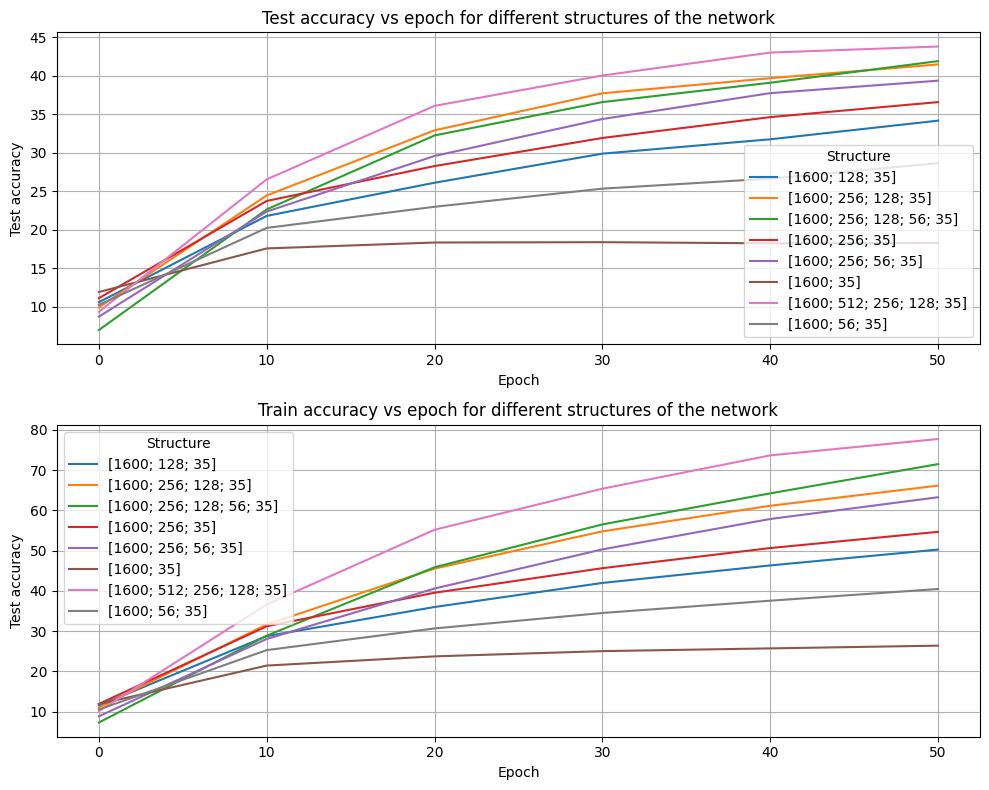
\includegraphics[width=.8\columnwidth]{images/diff_structures.png}
  \caption{Train and test accuracies for different network architectures}
  \label{fig-3}
\end{figure}

\subsection{Choice of the optimal lambda}

\begin{figure}[h]
  \centering
  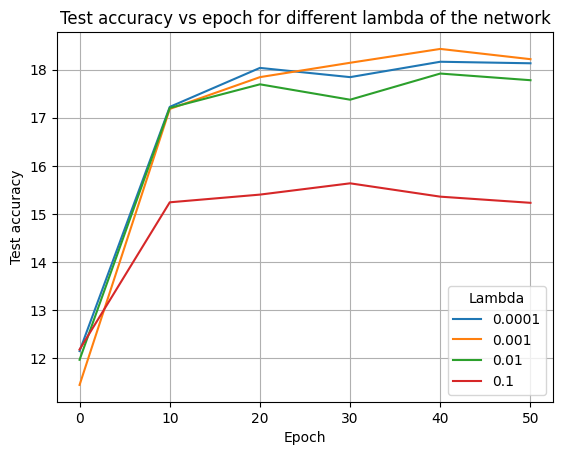
\includegraphics[width=.6\columnwidth]{images/lamda.png}
  \caption{Test accuracy for different lambda values}
  \label{fig-4}
\end{figure}
\subsection{Optimal network}
\rowcolors{2}{green!8}{green!18}
\begin{table}[H]
  \centering
  \begin{tabular}{|c|c|}
    \hline
    \linewidth=0cm
    Name server       & ip              \\
    \hline
    Google            & 8.8.4.4         \\
    Quad9             & 149.112.112.112 \\
    OpenDNS           & 208.67.220.220  \\
    Comodo Secure DNS & 8.20.247.20     \\
    \hline
  \end{tabular}
  \caption{Best neural network characteristics}
  \label{tab-1}
\end{table}
\section{Model analysis}
\begin{figure}[h]
  \centering
  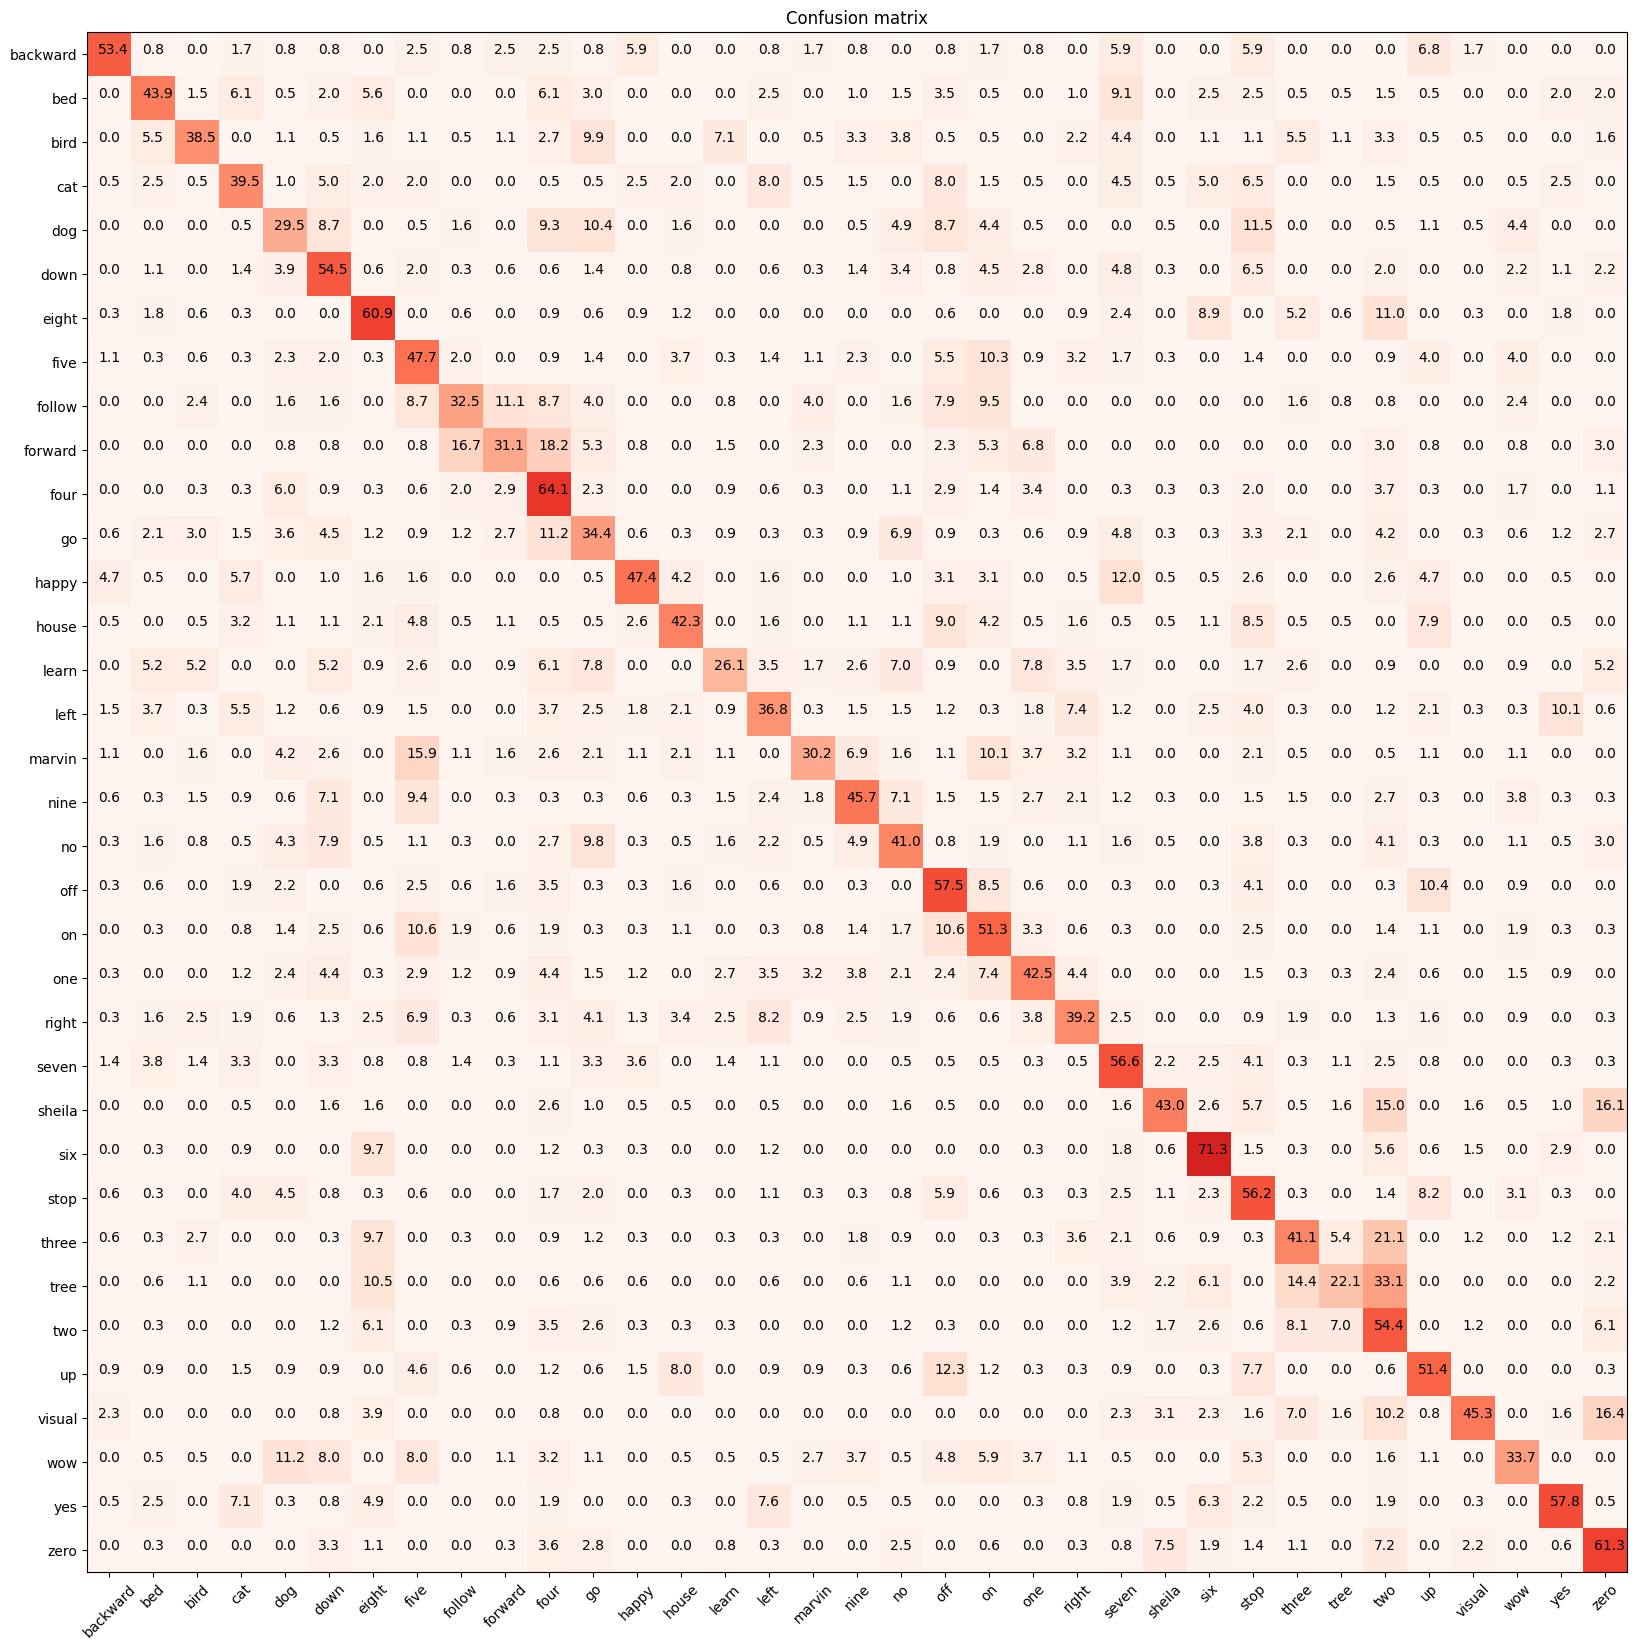
\includegraphics[width=.6\columnwidth]{images/confusion_matrix.png}
  \caption{Confusion matrix of the best model}
  \label{fig-5}
\end{figure}

\begin{figure}[h]
  \centering
  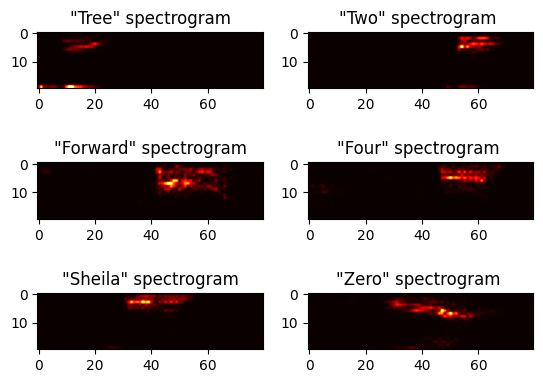
\includegraphics[width=.6\columnwidth]{images/misclassified_words.png}
  \caption{Spectrogram of the most 3 misclassified words, on left the correct word, on right the confused one}
  \label{fig-6}
\end{figure}

\section{Feature normalization}
\begin{figure}[h]
  \centering
  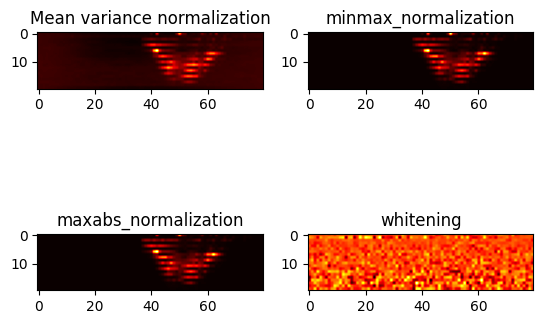
\includegraphics[width=.6\columnwidth]{images/normalization_spectrogram.png}
  \caption{Spectrogram of a sample of the dataset after different normalizations}
  \label{fig-7}
\end{figure}

\begin{figure}[h]
  \centering
  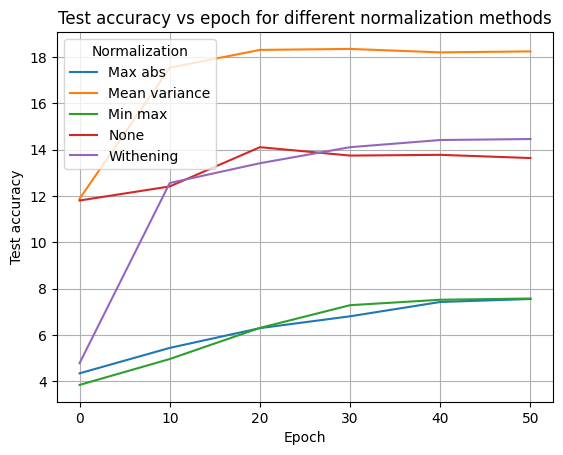
\includegraphics[width=.6\columnwidth]{images/test_diff_normalizations.png}
  \caption{Test accuracy for different normalizations}
  \label{fig-8}
\end{figure}
\section{Weights visualization}
\begin{figure*}[h]
  \centering
  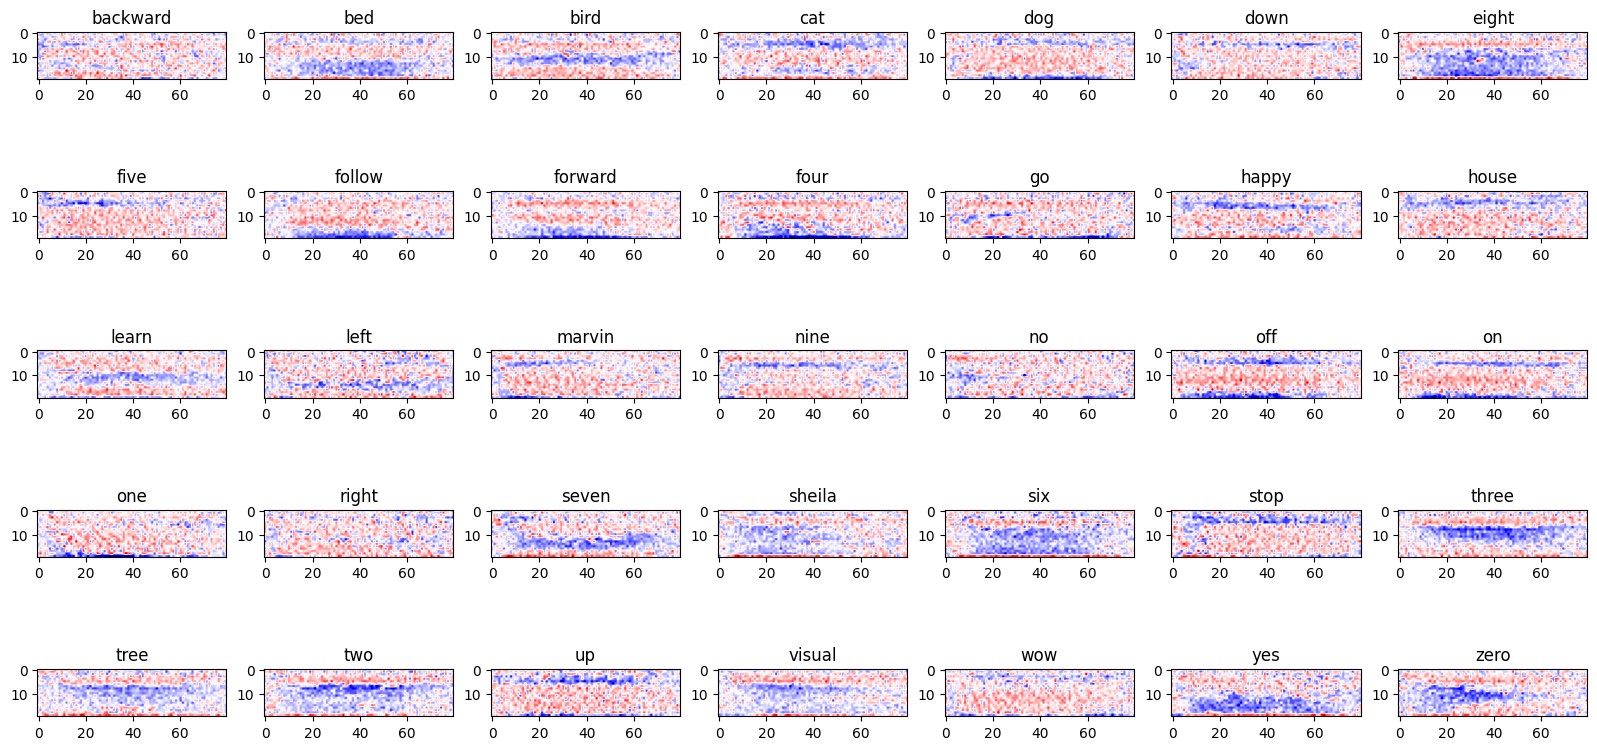
\includegraphics[width=0.8\linewidth]{images/spectrogram_weights.png}
  \caption{spectrogram of the weights of the output layer}
  \label{fig-9}
\end{figure*}

\end{document}